\documentclass[handout]{beamer}
\usepackage{graphicx}
\usepackage{algorithm}
\usepackage{algpseudocode}
\usetheme{PaloAlto}
\usecolortheme{rose}
\setbeamercovered{transparent}

\title{Portfolio Optimisation with SMC}
\author{Yow Tzu Lim, Nikolas Kantas}

\begin{document}
\begin{frame}
\maketitle
\end{frame}

\section{Overview}
\begin{frame}{Overview}
\begin{block}{Outline}
\begin{enumerate}
\item An introduction to Portfolio Optimisation.
\item Portfolio Optimisation as a Stochastic Control Problem.
\item Stochastic Control Problem as a Filtering Problem.
\item Sequential Monte Carlo (SMC) as an optimiser.
\item Model Control Predictive (MPC) to provide feedback.
\end{enumerate}
\end{block}
\begin{block}{Format}
$20-25$ mins \emph{interactive} session, interrupt and ask.
\end{block}
\end{frame}

\section{Portfolio Optimisation}
\begin{frame}{Maximising Returns}
  \begin{figure}
    \centering
    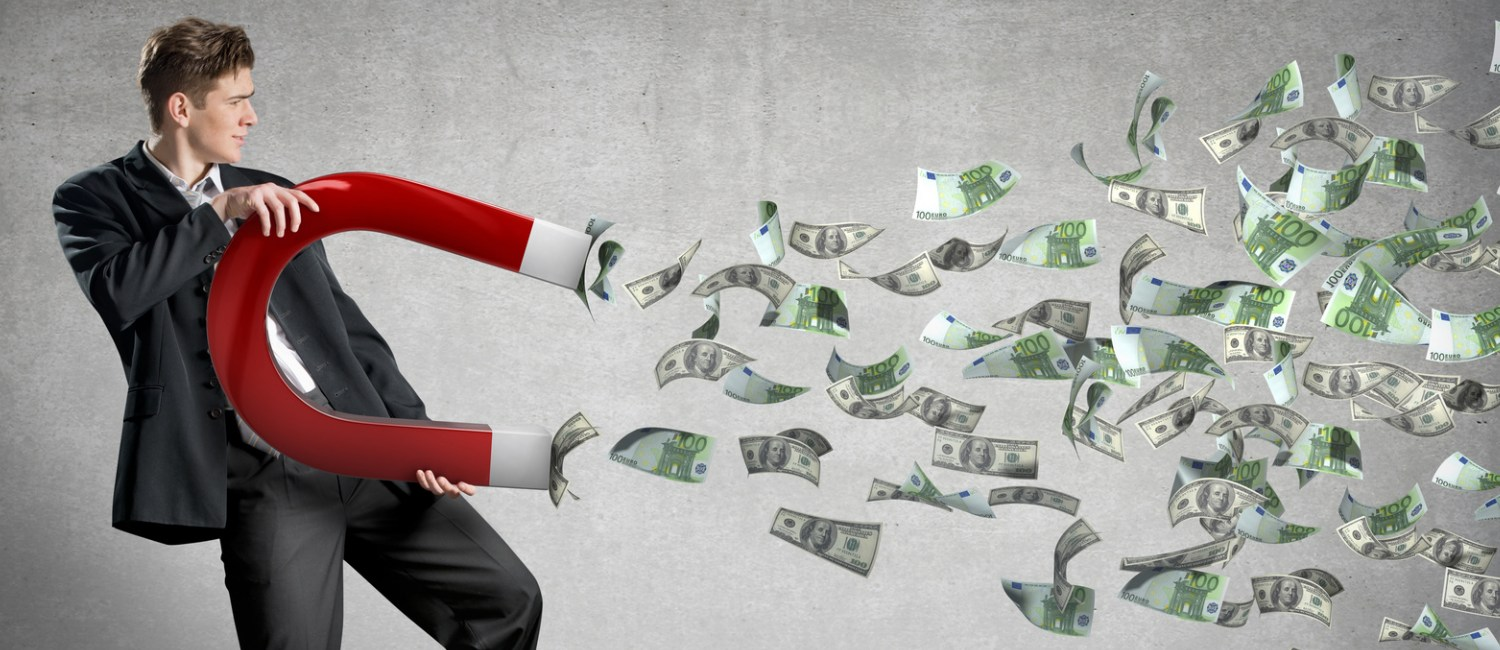
\includegraphics[width = 0.9\textwidth]{figures/magnetmoney.jpg}
    %\caption{Awesome figure}
  \end{figure}
\end{frame}

\begin{frame}{Minimising Risk}
  \begin{figure}
    \centering
    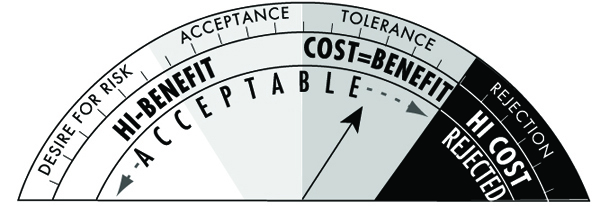
\includegraphics[width = 0.9\textwidth]{figures/risk.jpg}
    %\caption{Awesome figure}
  \end{figure}
\end{frame}

\begin{frame}{All eggs in one basket is too risky}
  \begin{figure}
    \centering
    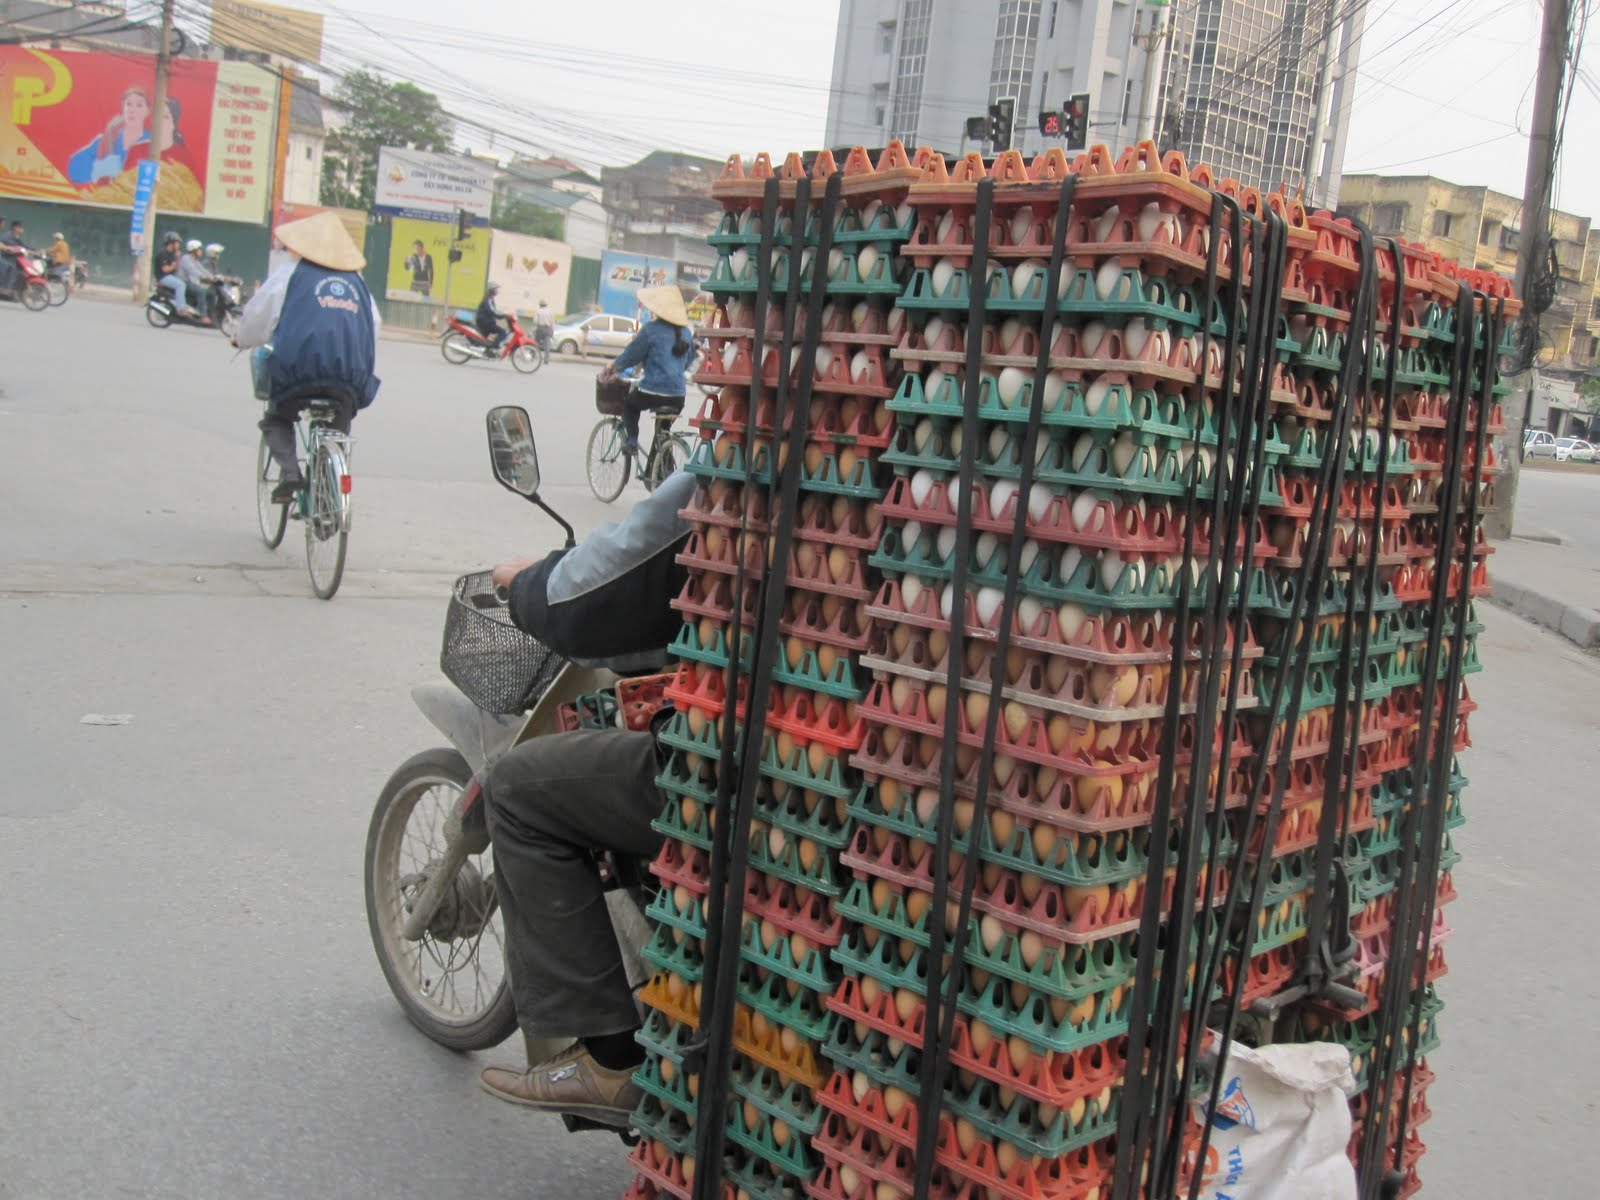
\includegraphics[width = 0.9\textwidth]{figures/alleggs.jpg}
    %\caption{Awesome figure}
  \end{figure}
\end{frame}

\begin{frame}{Diversification}
  \begin{figure}
    \centering
    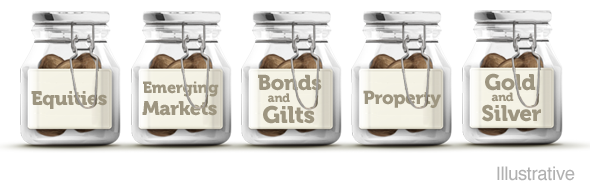
\includegraphics[width = 0.9\textwidth]{figures/allegg2.png}
    %\caption{Awesome figure}
  \end{figure}
\end{frame}

\begin{frame}{Modern Portfolio Theory}
  \begin{figure}
    \centering
    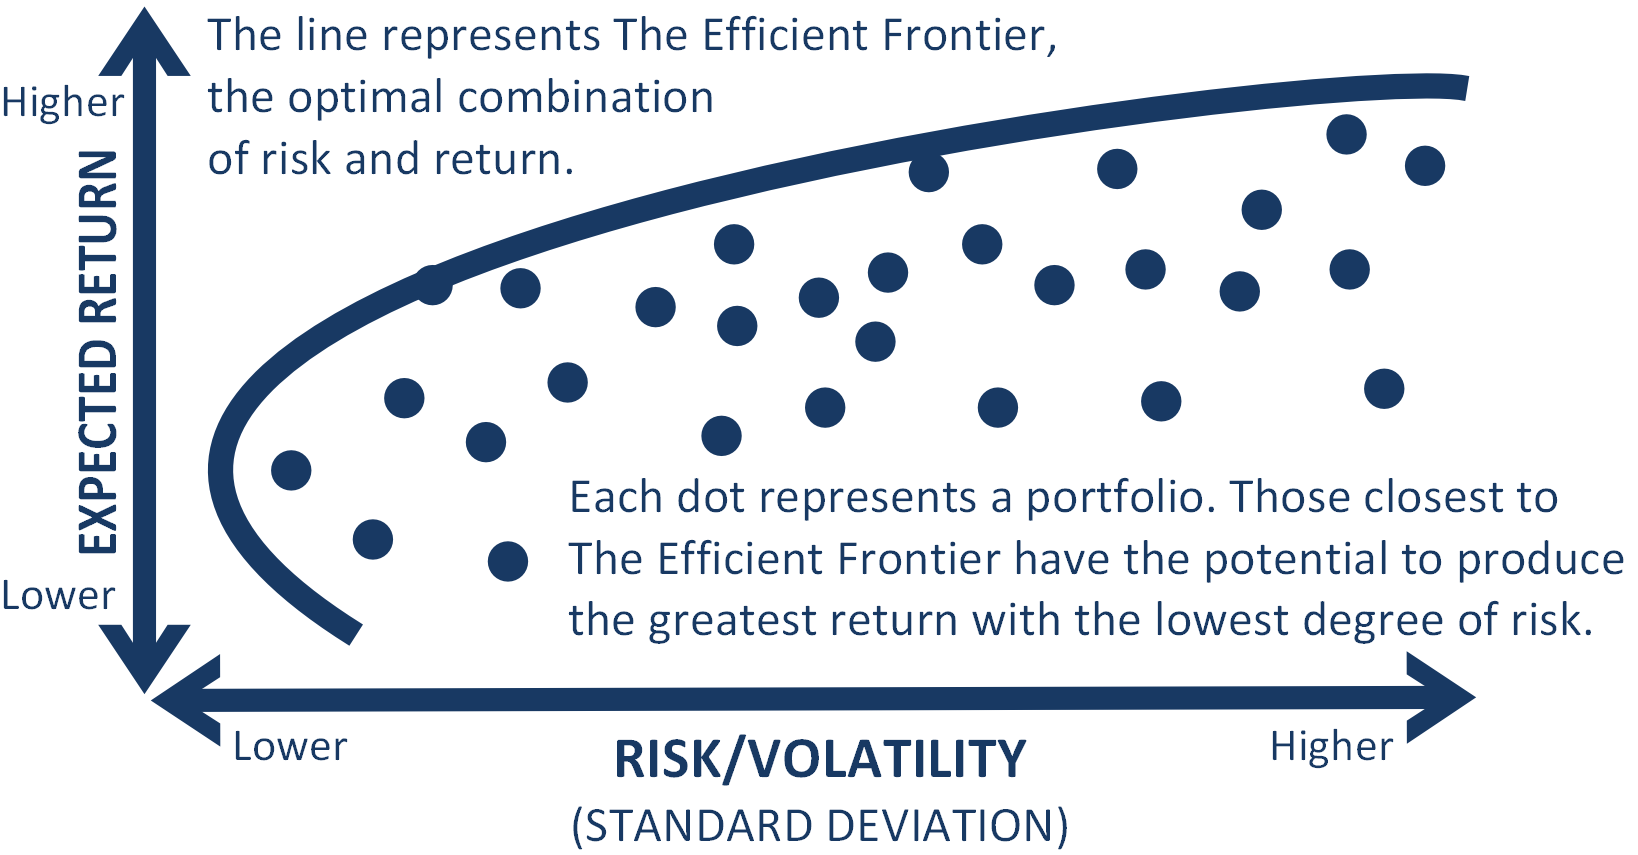
\includegraphics[width = 0.9\textwidth]{figures/mpt.png}
    %\caption{Awesome figure}
  \end{figure}
\end{frame}

\begin{frame}{A tale of two investment styles}
  \begin{figure}
    \centering
    \includegraphics[width = 0.7\textwidth]{figures/ap.jpg}
    %\caption{Awesome figure}
  \end{figure}
\end{frame}

\begin{frame}{S\&P Index for the last 5 Year}

  \begin{figure}
    \centering
    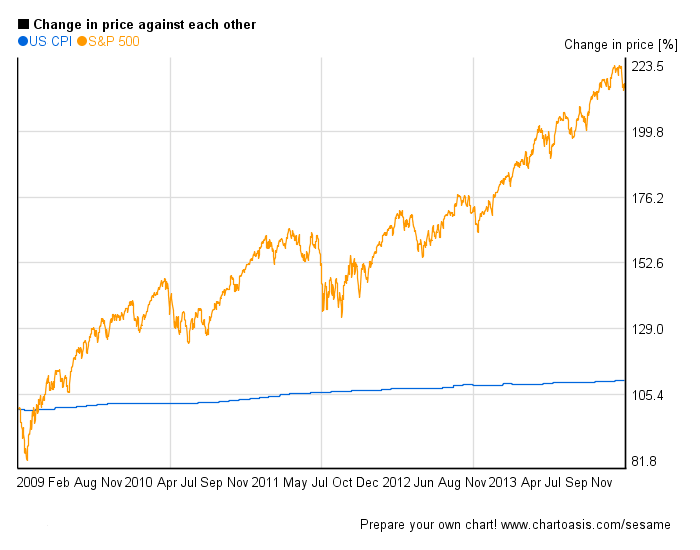
\includegraphics[width = 0.9\textwidth]{figures/snp500.png}
    %\caption{Awesome figure}
  \end{figure}

\end{frame}

\begin{frame}{Why Passive Index Fund?}
   \begin{enumerate}
\item Transparent and simpler.
\item Lower fees.
\item Less vulnerable to the change of managers.
\item Typically more tax efficient.
\item Comparable performance?
\end{enumerate}
\end{frame}

\begin{frame}{The infamous Vanguard Index Fund}
   \begin{figure}
    \centering
    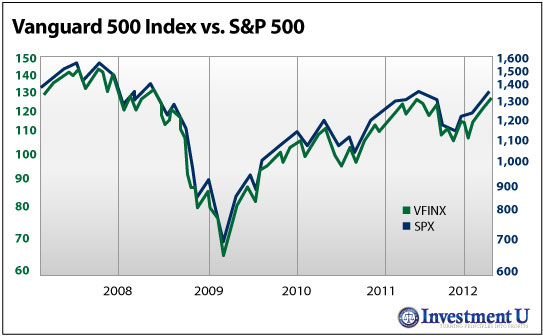
\includegraphics[width = 0.9\textwidth]{figures/vanguard.jpg}
    %\caption{Awesome figure}
  \end{figure}
   \ 
\end{frame}


\begin{frame}{The infamous Vanguard Index Fund}
   \begin{figure}
    \centering
    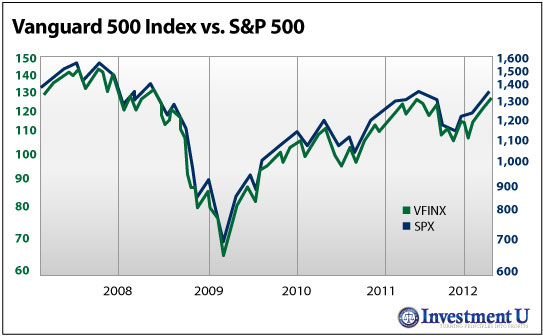
\includegraphics[width = 0.9\textwidth]{figures/vanguard.jpg}
    %\caption{Awesome figure}
  \end{figure}
  Replication is never perfect!
\end{frame}

\begin{frame}{Objectives}
\begin{enumerate}
\item Minimising the tracking error, $\epsilon$ of index tracking fund:
\begin{equation*}
\epsilon = \sqrt{Var[r_p - r_b]}
\end{equation*}
where $r_p$ is the return of the fund and $r_b$ is the return of the benchmark index.
\item Minimising the transaction costs.
\end{enumerate}
\end{frame}

\section{Methodology}

\begin{frame}{Time varying controlled HMM}
\begin{block}{Notation}
\begin{itemize}
\item $U_t$  --- proportion of each asset in portfolio
\item $X_t$ --- vector of prices of different assets
\item $Y_t$ --- index price
\end{itemize}
\end{block}
\begin{block}{Open Loop Policies}
\begin{itemize}
\item Express the objectives as a total \emph{reward} function $J_{x_0}(u_{1:T})$.
\item For an investment period $T$,  compute in one go at $t=0$:
   \begin{equation*}
      u^*_{1:T} = \arg\max J_{x_0}(u_{1:T})
   \end{equation*}
\item Easy but conservative.
\item Does not take into account $y_{1:t}, u_{1:t}$ at each time $t$.
\item A possible extension: MPC (see later).
\end{itemize}
\end{block}
\end{frame}

\begin{frame}{Time varying controlled HMM}
  \begin{figure}
    \centering
    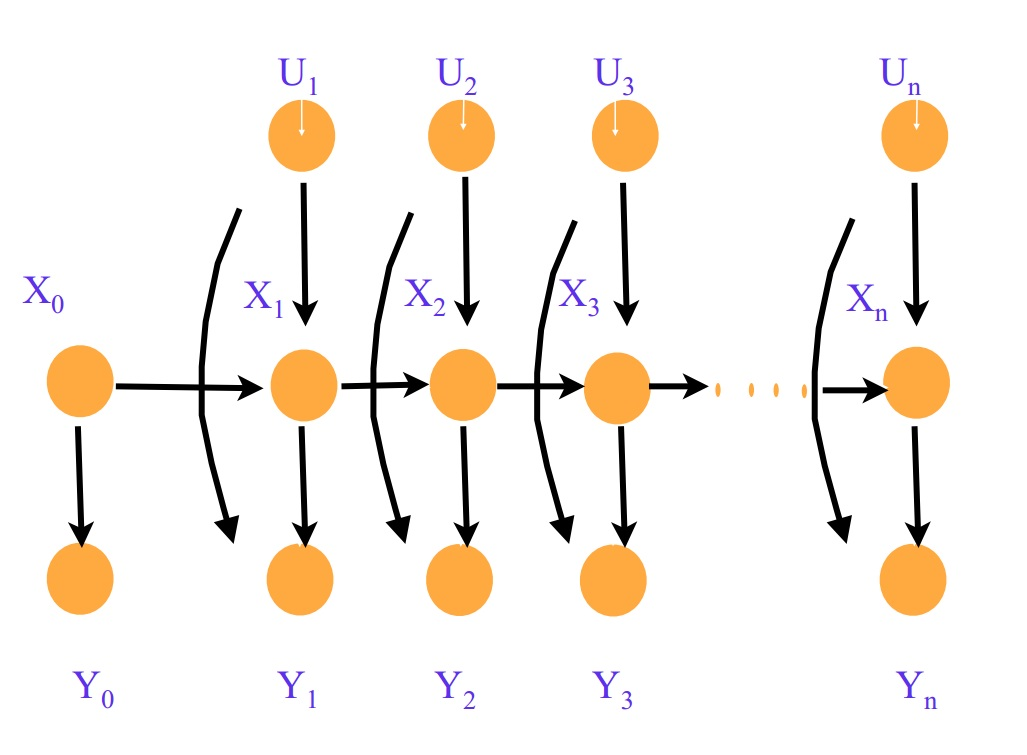
\includegraphics[width = 0.9\textwidth]{figures/hmm.jpg}
    %\caption{Awesome figure}
  \end{figure}
\end{frame}

\begin{frame}{Conditional Linear Gaussian Model}
\begin{block}{State-space Model}
\begin{align*}
  X_t &= A_t(U_t)X_{t-1} + B_t(U_t)W_t + F_t(U_t) \nonumber \\
  Y_t &= C_t(U_t)X_t + D_t(U_t)V_t + G_t(U_t)
\label{eq:model}
\end{align*}
where $W_t, V_t \sim \mathcal{N}(0,I)$.
\end{block}
\begin{block}{Transition Density and Conditional Likelihood}
\begin{align*}  p_t(u_t \mid u_{t-1}) &= \textrm{(any given form)} \nonumber \\
  f_t(x_t \mid x_{t-1}, u_t) &= \mathcal{N}(A_t(u_t) x_{t-1} + F_t(u_t), B_t(u_t)B_t(u_t)^T) \nonumber \\
  g_t(y_t \mid x_t, u_t)    &= \mathcal{N}(C_t(u_t) x_t + G_t(u_t), D_t(u_t)D_t(u_t)^T)
\end{align*}
Bayesian filtering can be computed using Kalman recursions.
\end{block}
\end{frame}

\begin{frame}{Open loop problem regulation}
\begin{block}{A multiplicative reward function}
\small
 $J(u_{1:T},y^{ref}_{1:T}, x_0)$ = 
\begin{equation*}
E_{x_0}\left[\exp\left( -\dfrac{1}{2}\displaystyle\sum^T_{t=1}\vert\vert y^{ref}_t - C_t(u_t)x_t - G_t(u_t) \vert\vert^2_{Q_t(u_t)^{-1}}  + \vert\vert u_t - u_{t-1} \vert\vert^2_{L_t} \right) \right]
\end{equation*}
where $\vert\vert x \vert\vert$ is the Mahalanobis distance, $Q(u_t) = D_t(u_t)D_t(u_t)^T$ and $L_t$ are assumed to known.
\end{block}
\begin{block}{Interpretation}
\begin{enumerate}
\item First term --- minimising the tracking error
\item Second term --- minimising the transaction cost
\item The corresponding optimal open loop policy is:
\begin{equation*}
  u^*_{1:T} = \arg\max_{u_{1:T}} J(u_{1:T};y^{ref}_{1:T};x_0)
\label{eq:optcontrol}
\end{equation*}
\end{enumerate}
\end{block}
\end{frame}

\begin{frame}{Problem Formulation}
\begin{enumerate}
\item Assume $\{U_t\}_{t \geq 0}$ is a Markov process with transition distribution $p(u_t \mid u_{t-1})$.
\item Calculate the marginal posterior distribution density:
\begin{equation*}
 \pi_t(u_{1:t}) = p(u_{1:t} \mid y^{ref}_{1:t})
\end{equation*} 
\item This can be obtained by marginalising the distribution $p(x_{1:t}, u_{1:t} \mid y_{1:t})$ which satisfies the following recursions:
\begin{align*}
  p(x_{1:t}, u_{1:t} \mid y_{1:t}) = &p(x_{1:t-1}, u_{1:t-1} \mid y_{1:t-1}) \times \\ &\frac{p(y_t \mid x_t, u_t)p(x_t, u_t \mid x_{t-1}, u_{t-1})}{p(y_t \mid y_{1:t-1})}
\end{align*}
\item Use Rao-Blackwellised SMC to model the states.
\item Compute the MAP estimate: $\hat{u}^*_{1:t} =  \arg\max_{u_{1:t}} p(u^{(i)}_{1:t} \mid y^{ref}_{1:t})^\gamma,~\gamma > 0$.
\end{enumerate}
\end{frame}

\begin{frame}{Intro to SMC in 1 minute}
  \begin{figure}
    \centering
    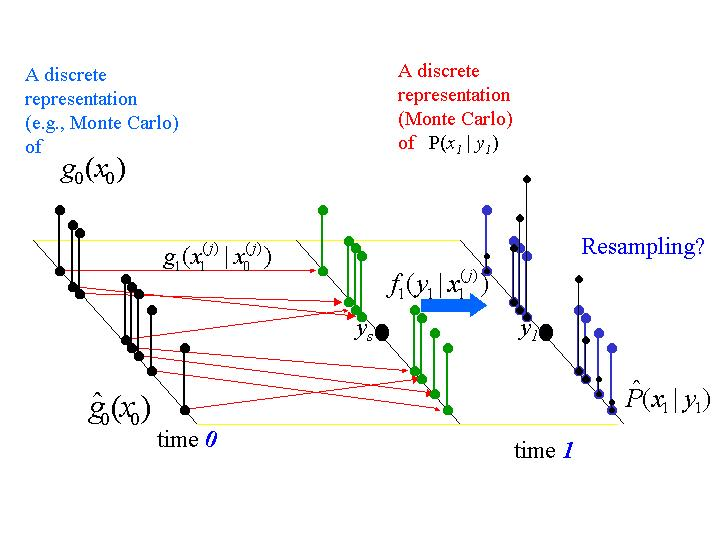
\includegraphics[width = 0.9\textwidth]{figures/pfilter.jpg}
    %\caption{Awesome figure}
  \end{figure}
\end{frame}

\begin{frame}{The duality of the two problems}
Putting all these together, we have the following:
\begin{equation*}
  u^*_{1:t} = \tilde{u}^*_{1:t} = \arg\max_{u_{1:t}} \pi_t(u_{1:t})^\gamma,~\gamma > 0
\end{equation*}
In SMC algorithm, this can be easily estimated as follows:
\begin{equation*}
\hat{u}^*_{1:t} = arg\max_{u_{1:t}} \pi_t(u^{(i)}_{1:t})^\gamma = \arg\max_{u_{1:t}} p(u^{(i)}_{1:t} \mid y^{ref}_{1:t})^\gamma
\end{equation*}
\end{frame}

\section{Simple Experiment}
\begin{frame}{Tracking an oscillating wave}
\begin{block}{The state space model}
  $X_t = X_{t-1} + W_t + U_t, W_t \sim \mathcal{N}(0,I)$
  $Y_t = X_t + V_t, V_t \sim \mathcal{N}(0,I)$
\end{block}

\begin{block}{Target reference signal}
$y^{ref}_t = \cos(0.2 \pi t + 0.3)$ 
\end{block}

\begin{block}{Parameter Settings}
\begin{enumerate}
\item Various time period length, $T$: 5, 10 and 20.
\item Various sample size, $N$: 100, 500, 1000, 5000 and 10000.
\item Resampling step: Always vs. Selectively with ESS.
\item Resample-Move step with MCMC (random walk proposal).
\item Various $\gamma$ settings: Constant function of $1$, $50$, $100$, $1000$ and increasing function of time $t$, $10t$, $50t$ and $100t$.
\end{enumerate}
\end{block}
\end{frame}

\begin{frame}{ Results and Discussion}
\begin{enumerate}
\item More samples helps --- better distribution representation
\item ESS doesn't help --- resampling pushes samples towards the mode
\item MCMC helps --- introduce diversity to counter sample degeneracy
\item $\gamma$ setting need tuning --- optimisation vs. exploration
\end{enumerate}

  \begin{figure}
    \centering
    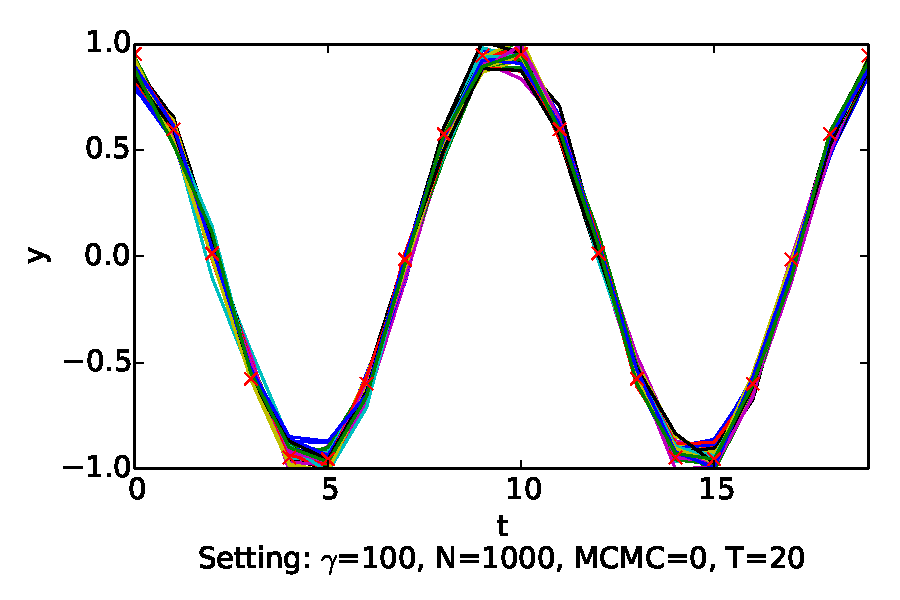
\includegraphics[width = 0.7\textwidth]{figures/output_y/output_20_100.pdf}
    %\caption{Awesome figure}
  \end{figure}
\end{frame}

\section{Real-World Application}
\begin{frame}{Tracking the DAX Index}
\begin{block}{the DAX Index}
\begin{enumerate}
\item One of the major index of the world
\item 30 largest companies in Germany as the constituents
\item Data: Adjusted daily close from Jan 2014
\end{enumerate}
\end{block}
\begin{block}{Experiments}
\begin{enumerate}
\item DAX4
\item DAX with full replication
\item DAX with partial replication
\item DAX with MPC
\end{enumerate}
\end{block}
\end{frame}

\begin{frame}{The state space model}
\begin{align*}
  X_t &= X_{t-1} + F_t(U_t) + W_t \\
  Y_t &= 30U^T_tX_t + 0.01V_t
\end{align*}
where
\begin{itemize}
\item $W_t \sim \mathcal{N}(\mu_{t_0}, \Sigma_{t_0})$, $V_t \sim \mathcal{N}(0, I)$
\item $\{X_t\}_{t \geq 0}$ is a vector of stock price processes modelled as Arithmetic Brownian Motion with drift
\item $\{U_t\}_{t \geq 0}$ is a vector represents the stock positions
\item $F_t(U_t)$ can be viewed as the market impact on prices
\item $\mu_{t_0}$ and $\Sigma_{t_0}$ are vector of the EWMA estimated mean and covariance matrix of the price changes
\item $\{Y_t\}_{t \geq 0}$ is the process represents the index level.
\end{itemize}
\end{frame}

\begin{frame}{Results of Full Replication}
   \begin{figure}
    \centering
    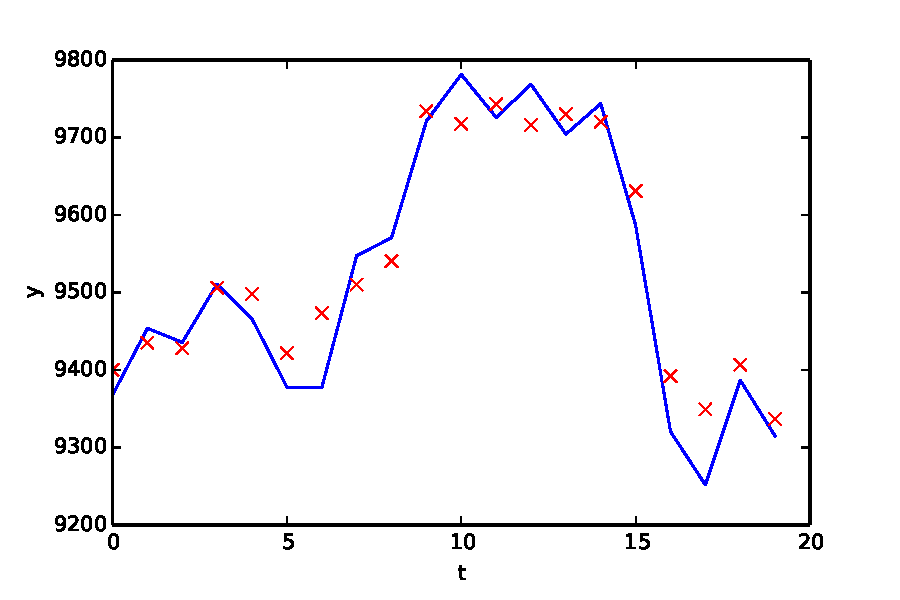
\includegraphics[width = 0.9\textwidth, height=0.4\textheight]{figures/DAXFull-y.pdf}\\
    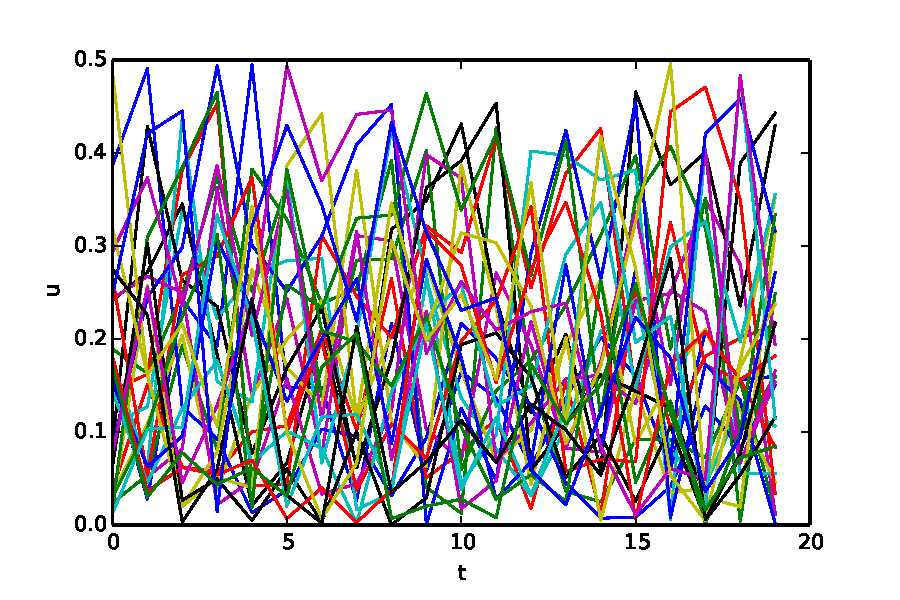
\includegraphics[width = 0.9\textwidth, height=0.4\textheight]{figures/DAXFull-u.pdf}
   \end{figure}
\end{frame}


\begin{frame}{Results of Partial Replication using top 6 stocks}
   \begin{figure}
    \centering
    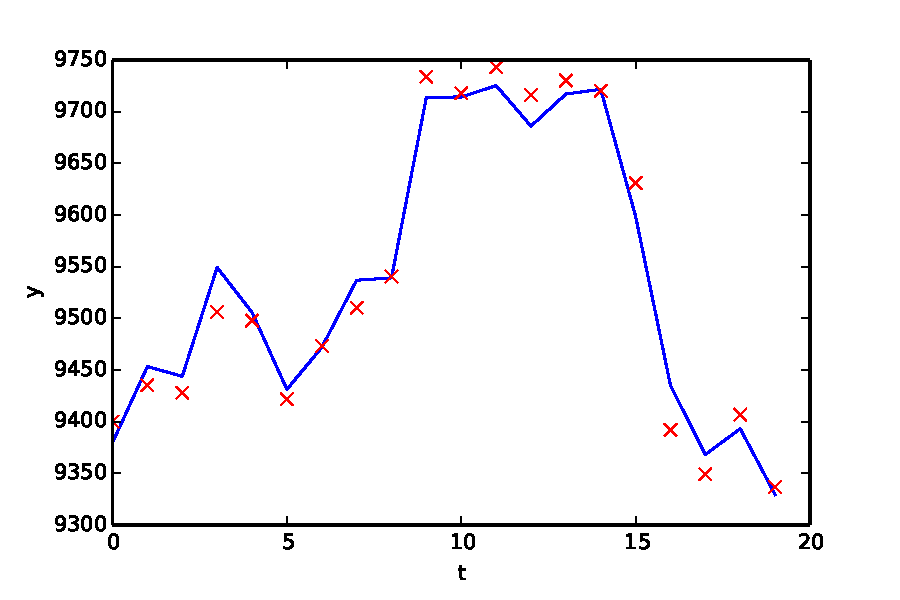
\includegraphics[width = 0.9\textwidth, height=0.4\textheight]{figures/DAXPartial-y.pdf}\\
    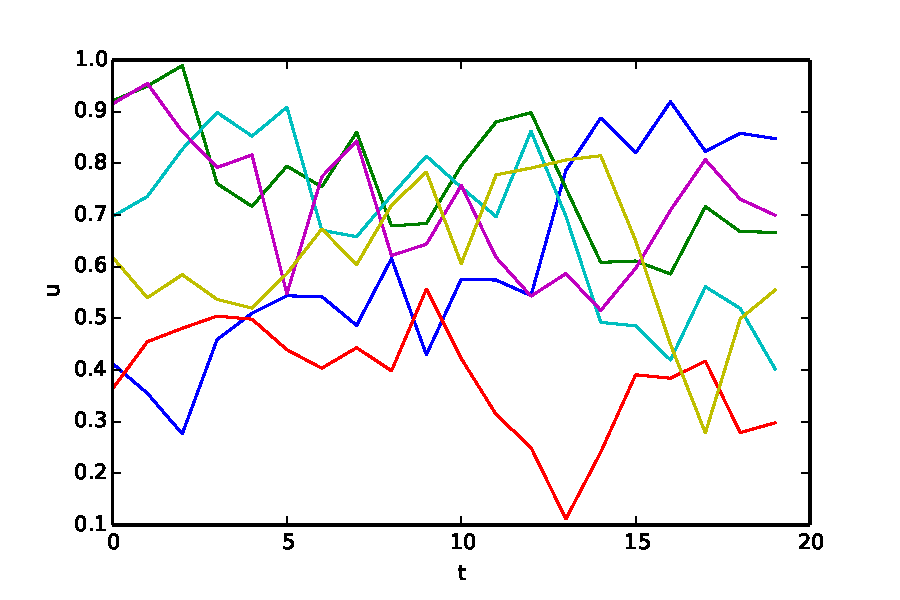
\includegraphics[width = 0.9\textwidth, height=0.4\textheight]{figures/DAXPartial-u.pdf}
	\end{figure}
\end{frame}

\begin{frame}{Review}
\begin{block}{What we have achieved so far}
The technique is able to track a \emph{given} target reference index.
\end{block}

\begin{block}{Issues}
\begin{enumerate}
\item We do not have the reference signal for future time.
\item Open loop policy, no feedback used.
\end{enumerate}
\end{block}

\begin{block}{Solution}
\begin{enumerate}
\item use EWMA estimate for the target reference signal.
\item use Model Predictive Control (MPC).
\end{enumerate}
\end{block}
\end{frame}

\section{Model Predictive Control}
\begin{frame}{MPC: Algorithm}
  \begin{figure}
    \centering
    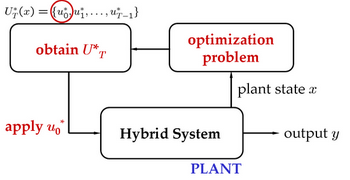
\includegraphics[width = 0.7\textwidth]{figures/mpc.png}
    %\caption{Awesome figure}
  \end{figure}

  \begin{algorithmic}[1]
  \State Set $t = 1$.
  \While{$t \leq T$}
  \State Search the optimal $u^*_{t:t+H}$ for the problem $t:t+H$.
  \State Apply the first set of the optimal control  $u^*_{t}$.
  \State Update the model states with any new information.
  \State Set $t = t + 1$.
  \EndWhile
  \end{algorithmic}
\end{frame}

\begin{frame}{MPC: T=20}

   \begin{figure}
    \centering
    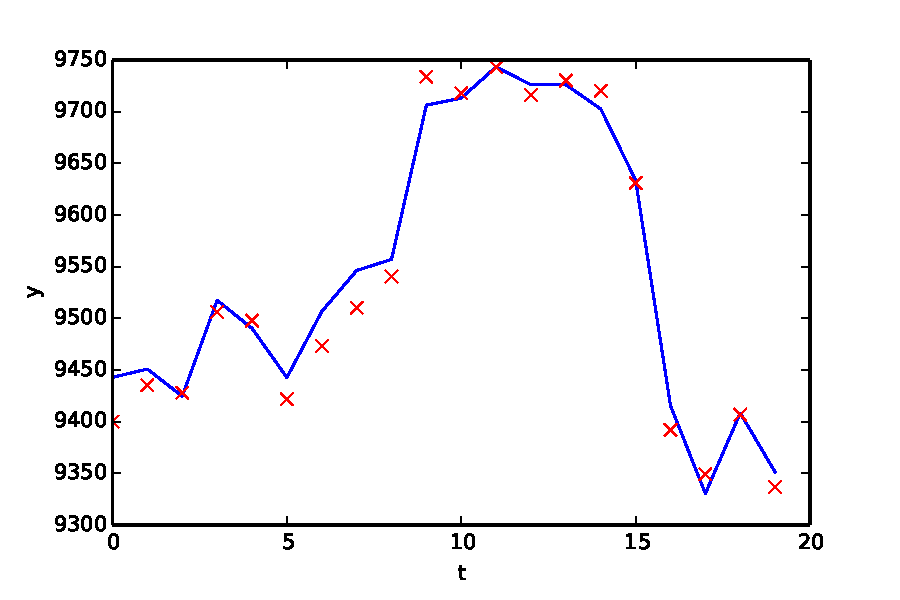
\includegraphics[width = 0.9\textwidth, height=0.4\textheight]{figures/DAXMPC-y-2.pdf}\\
    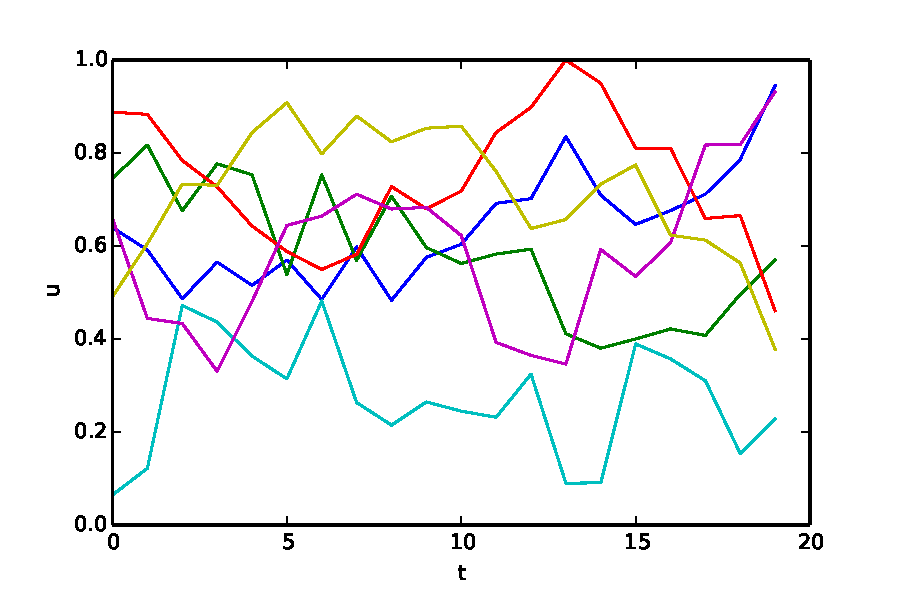
\includegraphics[width = 0.9\textwidth, height=0.4\textheight]{figures/DAXMPC-u-2.pdf}
  \end{figure}
\end{frame}


\begin{frame}{MPC: T=125}
   \begin{figure}
    \centering
    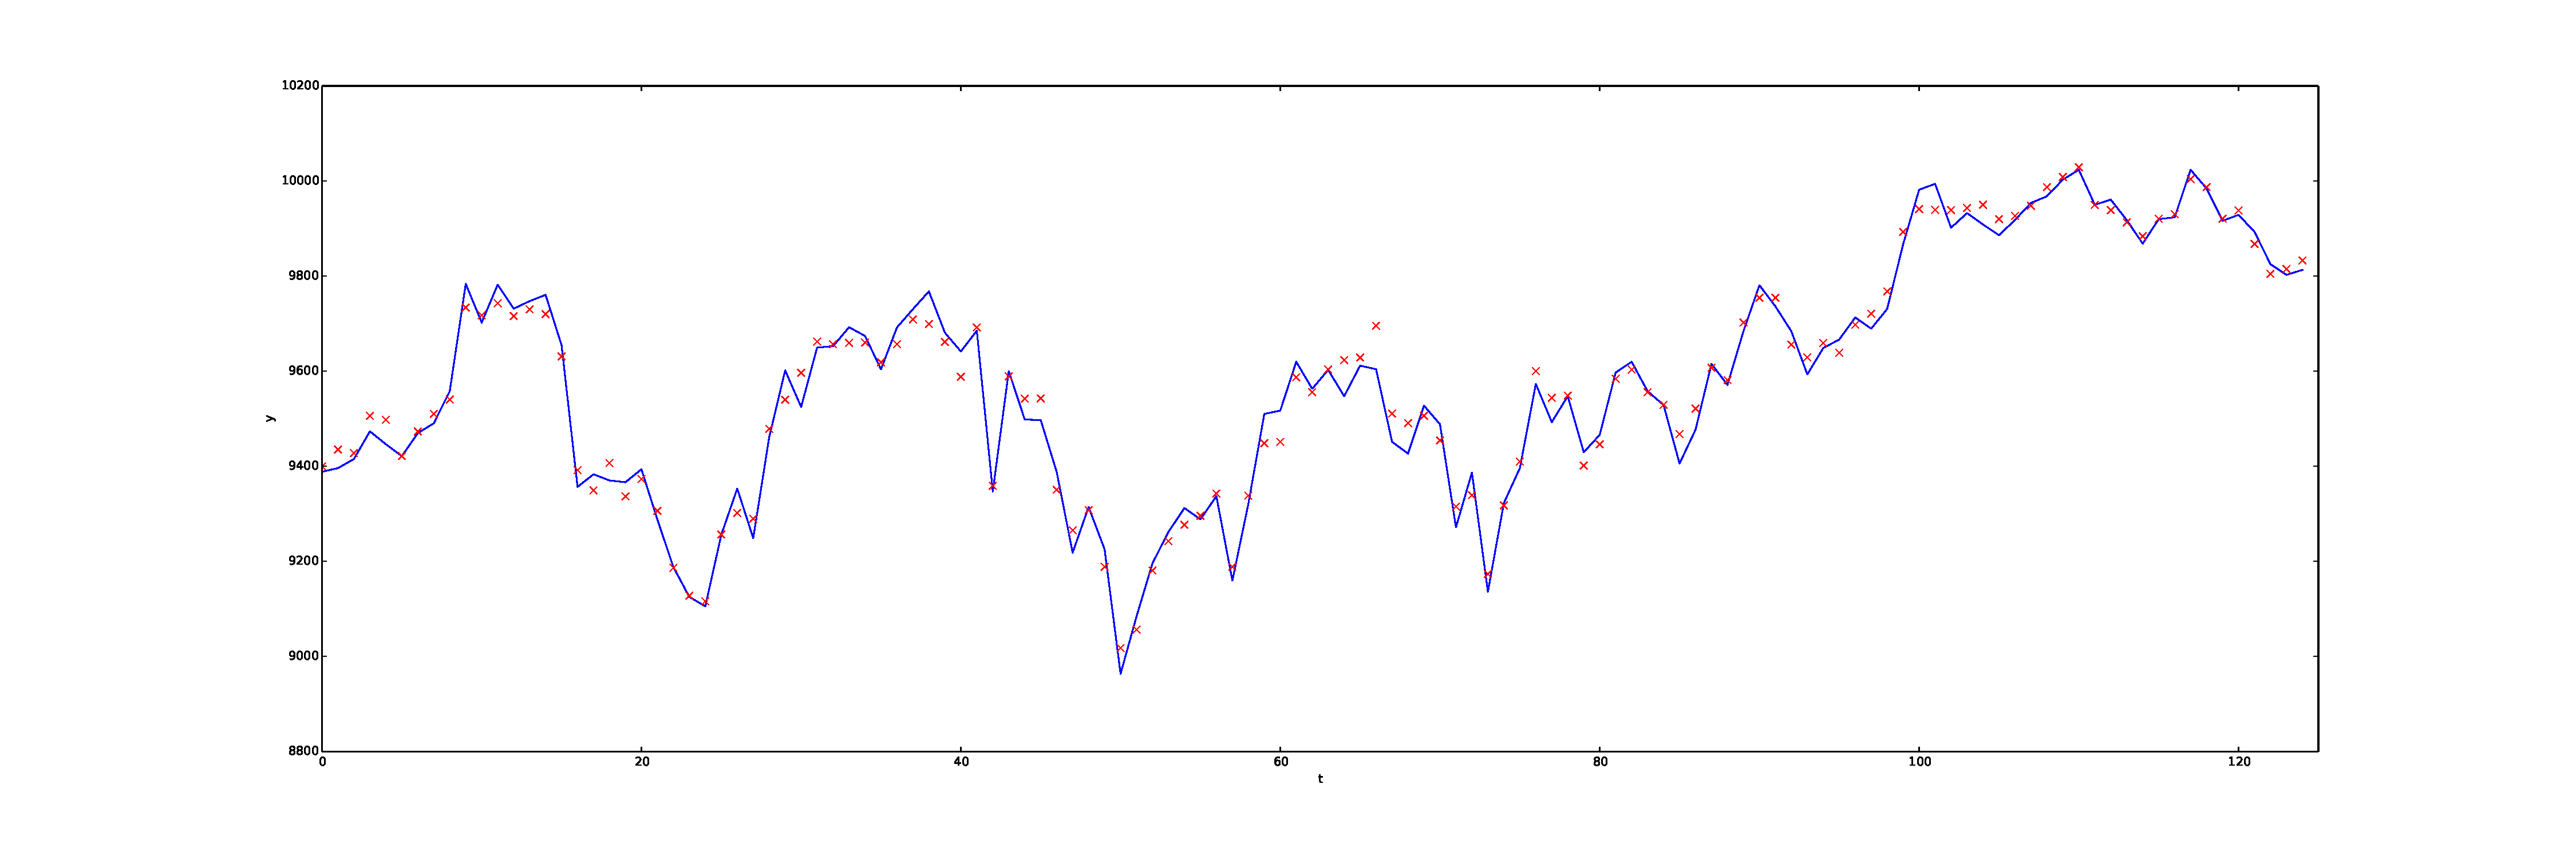
\includegraphics[width = 0.9\textwidth, height=0.4\textheight]{figures/DAXMPC-y-2-long.pdf}\\
    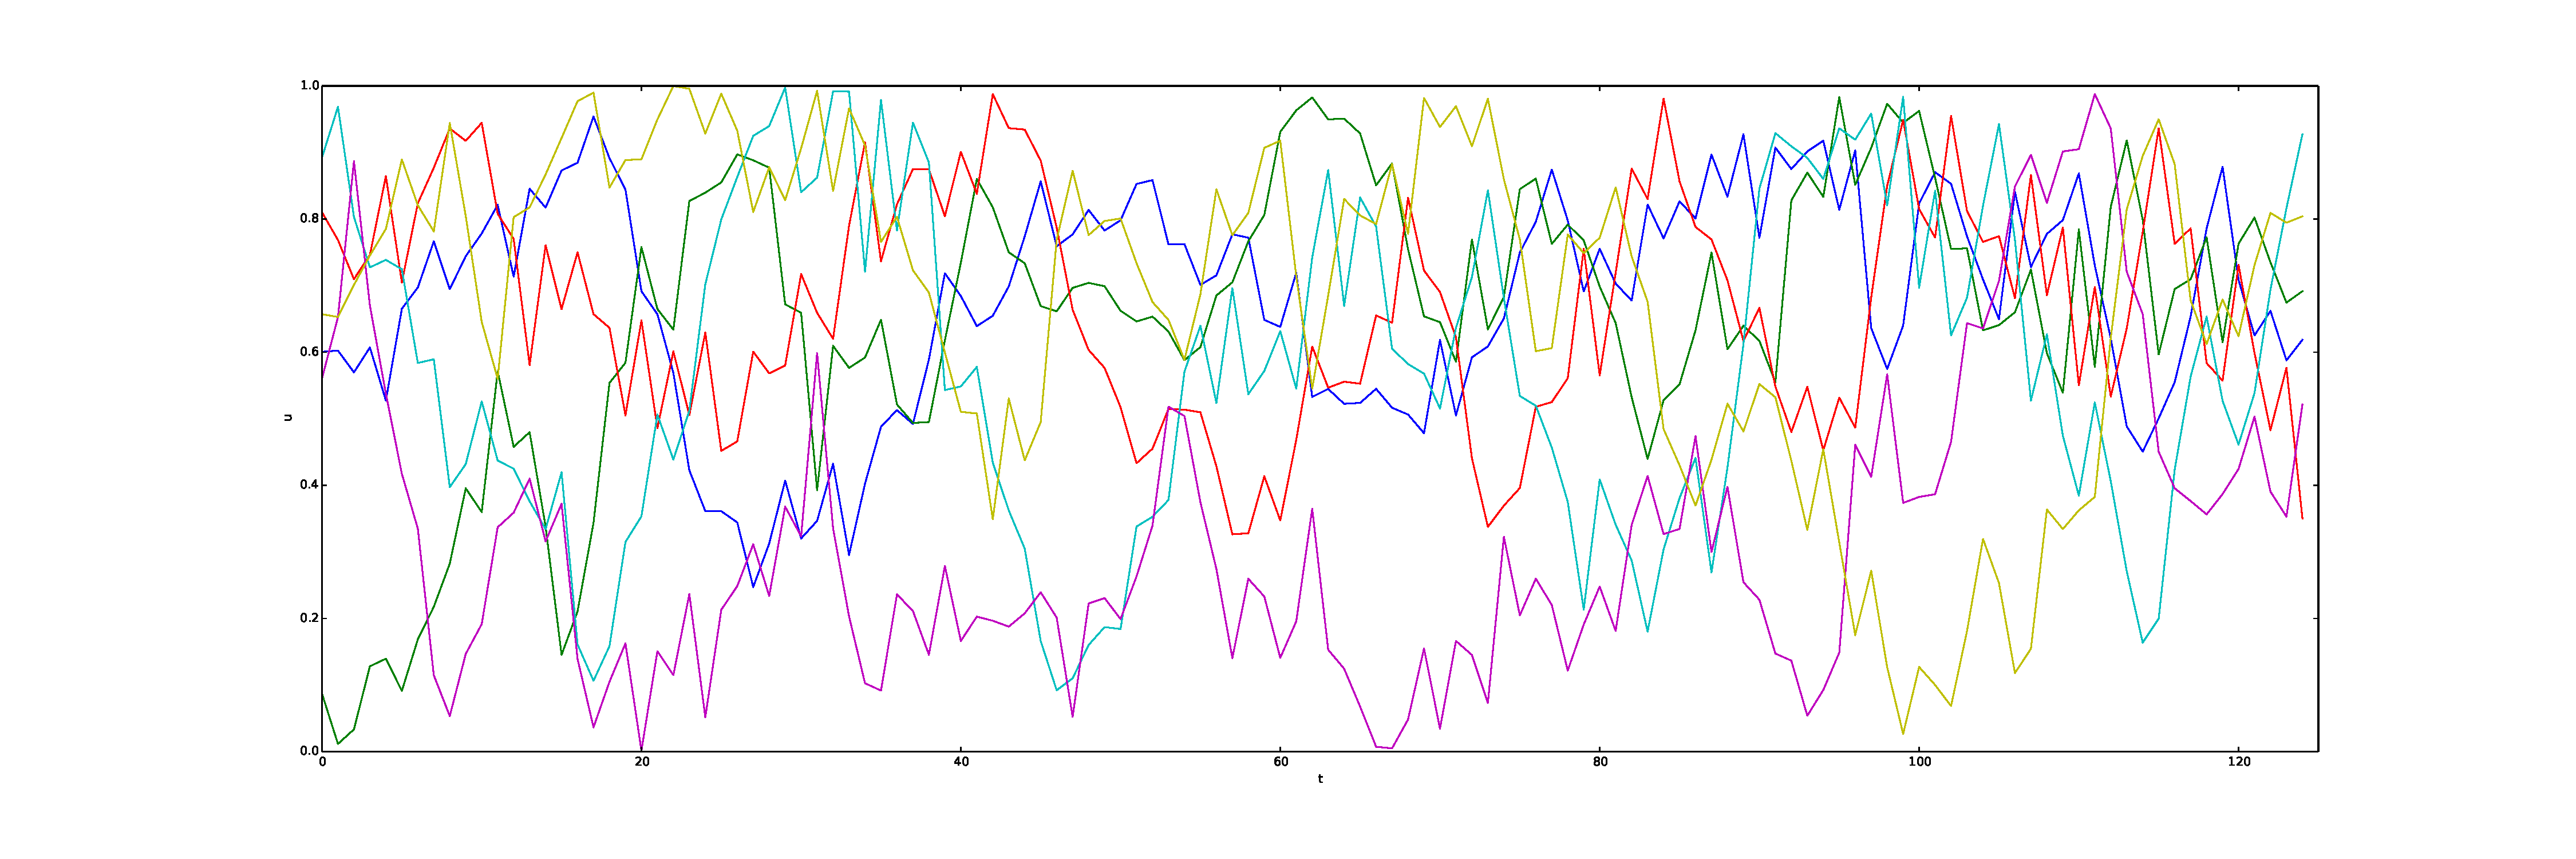
\includegraphics[width = 0.9\textwidth, height=0.4\textheight]{figures/DAXMPC-u-2-long.pdf}
  \end{figure}
\end{frame}

\section{Conclusions}
\begin{frame}{Contributions}
\begin{enumerate}
\item Portfolio optimisation problem $\rightarrow$ control problem $\rightarrow$ filtering problem $\rightarrow$ using SMC as a maximiser.
\item The sensitivity of SMC in terms of the parameter settings are explored, e.g., ESS should not be used, $\gamma$ setting, etc.
\item Demonstrate how the SMC technique proposed can be used in the MPC framework.
\end{enumerate}
\end{frame}

\begin{frame}{Future Work}
\begin{enumerate}
\item More realistic models.
  \begin{itemize}
   \item Geometric Brownian Model, Jump Diffusion model, etc.
   \item Moving away from a conditional Gaussian model \\$\implies$ the  Kalman Filter recursions is no longer optimal.
   \item Try $SMC^2$.
  \end{itemize}
\item Parallel computation.
  \begin{itemize}
   \item The nested SMC setup inevitably adds consideration amount of computation requirements. 
   \item Graphics Processing Units (GPU).
  \end{itemize}
\item More complex financial indices.
\end{enumerate}
\end{frame}

\begin{frame}{Questions?}
Thank you.
\end{frame}


\end{document}
